%Die Angabe des schlauen Spruchs auf diesem Wege funtioniert nur,
%wenn keine Änderung des Kapitels mittels den in preambel/chapterheads.tex
%vorgeschlagenen Möglichkeiten durchgeführt wurde.

\chapter{Concept}
\label{chap:concept}
%\vspace{-3cm}
%\vspace{2cm}

%abstrakte Beschreibung des Lösungsansatzes / der Lösungsansätze
This thesis engages with the process of creating interactive installations on ubiquitous displays especially on the creation and mobile adaption of its displaying content. Observations within the meSch EU project show that the current practice of cultural heritage professionals (CHPs) is to create and adjust content mostly on desktop computers and then deploy it remotely on a specific target display. Authors do often use multiple software combined to create simple content which makes it complex and costly. But content which seems well prepared on desktop computers may look completely incorrect on the target display. There are many different factors which influence the visual representation such as screen resolution, density, projection surface or viewing angle. Authors do therefore need to go through several time-inefficient cycles to get an acceptable but not a high quality result on the target display. 
Another difficult part of creating and deploying such installations is providing interactivity. The main question and barrier is how end-users such as CHPs can combine digital content to physical interaction. To achieve interactivity authors have to put in big cost and time effort because they do not have the needed expertise in programming or technical understanding by themselves and need to hire specialists.

So the current content creation, adaption and deployment process is not well adapted to its purpose (e.g prepare content different screen resolution) and misses some necessary features (e.g. providing interactivity in a simple and cost-efficient way). This thesis explores ways in which one single system is usable by authors without a higher technical understanding and not only by technical specialists to fill the missing gaps within the current approaches. Therefore, the first part is to minimize the technical boundaries for users. The goal is an approach which supports optimizing the process of creating and deploying content on a specific target device. Secondly the approach should enable on-site editing of content with immediate feedback of the changes and their representation on the target display. Thirdly there should be a way to combine physical interaction with digital interaction without big effort and technical expertise. This means, the approach should provide the possibility to modify content on the target display by using physical objects or sensors. In the following the requirements which were defined for the approach are explained in detail.

\section{Reducing technological complexity}
The approach should minimize the technical boundaries for an author to create an interactive installation. Therefore, a blackbox-system which, once installed, provides all the functionality to create interactive installations in an appealing and fast way should be provided. Additionally, the system must not need non-standard technical requirements which need massive adaptions or costly investments. Furthermore, creators should not need to have a technical understanding of the system. Content management systems in the field of web development seemed to be a good model where users do not need to know how the underlying technical part of the system and the technology works but they can create websites and content quick and easily. Using web technology for the toolkit colludes with the existing meSchup platform described in \cite{Kubitza2015n}. Developing the toolkit as a plugin for the meSchup platform supports the blackbox-approach and provides further possibilities for the communication between the two systems. The communication enables the interactivity between physical objects and digital content. Furthermore, through this plugin architecture an easy way to let authors create rules for interactive digital content should be provided.

\section{Content Creation}
The process of the content creation is an important step while establishing an interactive installation. Authors spend a lot of time searching and collecting content. The approach should therefore support authors while preparing these contents by providing one single system combining all the features needed to create appealing presentations. The approach should support the necessary media types which are used in interactive installations like text, images, audio and video as well as more complex content like content feeds or whole websites. Furthermorem, it should support managing added media in a way known by many content management system in the field of web development. Microsoft Powerpoint seems to be a good model where users create and present information in an appealing and structured way. Most creators know this system and feel comfortable with the way it works. Leaning on this approach seems to be a good approach to improve the user experience and to reduce the complexity of the system as well as the time users need to learn how to use it.
Assuming that viewers will be multilingual the toolkit should support translation of created content. 
 
\section{On-Site Editing}
To reduce the time needed to adapt an existing installation to the target environment our approach should support on-site editing of content with a mobile device. Visiting the installation and correcting its deficits on place will bring a big efficiency improvement to the creation- and adaption- as well as the deployment-process. Instead of constantly switching between desktop computer and deployment environment the author just needs to create the content once and adapt it on-site using a mobile device of its choice. A further advantage of the on-site editing is that the author can experience the deployed installation as a common visitor and therefore can adapt the presentation more appealing. 

\section{Interactivity Scripting}
An interactive installation is way more interesting, improves user experience, draws interest and provides more possibilities than a display with static information. The approach should give the users the ability to create interactive content as easy as static content. To achieve this the toolkit will be connected to the meSchup platform. Through this connection sensors and actuators are provided as trigger for the interactive content. Furthermore, the technical part of the meSchup platform should be hidden to provide the users a simple solution to create rules for interactive content. There should be an easy editor with drag and drop functionality to create rules without the need of programming skills as well as predefined templates from which users can choose matching templates according to their usage scenario and hardware. In detail there should be the possibility to create advanced behavior scripts written in JavaScript which are overlaid with semantic textual stories that embed form elements at specific positions to represent configurable parameters of the actual implementation. Using the text-based story together with control elements for customizing the behavior are a concept that is supposed to be well understandable by users without technical expertise. Those behavior scripts are provided by programmers and will be integrated into the system as behavior rule templates. Users then can choose from different templates and configure the parameters visible within the story of the behavior rule.

\section{Scenarios}
In the following section three different scenarios which illustrate our concept are presented. Firstly it is described how installation with digital content or interactive installations are created and used. Secondly an explanation is given why the toolkit will improve the current approaches in the given scenario.

\subsection{Scenario I - Cultural Heritage}
The first scenario is set in the field of cultural heritage especially about how museums create and make use of interactive installations with digital content. At first it is shown how curators create exhibitions with digital content based on observations of the meSch EU project. Secondly it will be explained how time-consuming and costly the creation of interactive installations for curators are at the current time. Afterwards an explanation of how exhibitions with digital content can be created within the VEII toolkit is given. Then it will be shown how the current creation and deployment process can be improved. At last it will be shown how the VEII toolkit will support curators to create interactive exhibitions easily and cost-efficient.

Observations within the meSch EU project showed that curators who want to create content for new exhibitions with digital content start at their desktop computer collecting and composing text and multimedia. Then they use software like Microsoft Word or Adobe Photoshop to prepare and arrange the content according to the installations purpose. After finishing the content creation and composing part at the desktop computer curators often need to export their content to a specific format (e.g. PDF) and deploy this file manually on the target computer (e.g by using a USB-stick or using a FTP-client) which is connected to the display device. If curators find content which is not well adopted for the target environment while examining the actual exhibition they need to go back to their desktop computer to adapt this specific content and repeat the whole deployment process. Often content creation/adaption-cycles (Figure~\ref{fig:cycle_1}) with many iterations arise in this occasion which are neither time-efficient nor produce a high content quality. 

\begin{figure}
  \begin{center}
    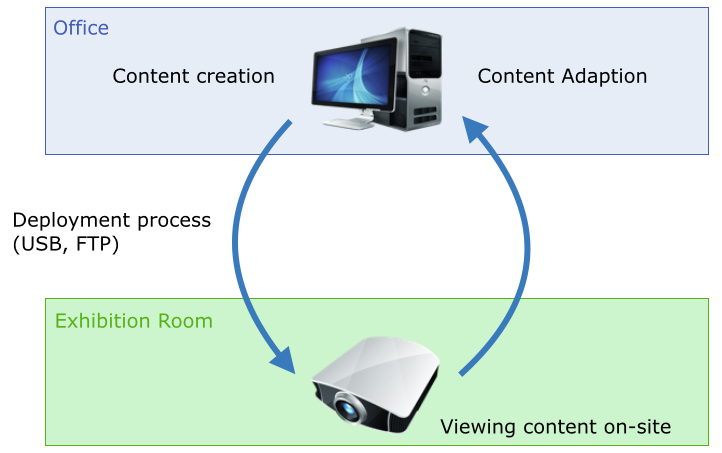
\includegraphics[width=0.8\textwidth]{cycle_1.png}
    \caption{The content creation/adaption cycle of cultural heritage professionals}
    \label{fig:cycle_1}
  \end{center}
\end{figure}

Curators are often limited in the creation of interactive exhibitions. They do not have the technical expertise as well as the needed hard- and software. So to deploy exhibitions with interactive digital content they need to hire specialists and/or buy particular software. Curators do therefor have to put big time- and cost-effort in those exhibitions for which reason they have to weigh up the cost and benefit for every new project. Furthermore, curators often cannot reuse most of the components used during the exhibition after it ended. 

With VEII realizing our on-site content editing approach as well as our interactivity scripting approach, the toolkit supports curators in creating interactive exhibitions with digital content in a more pleasant and effective way. By using the toolkit curators can compose content on their desktop computer as they are used to using the VEII web-based user interface. There they can create and adapt multimedia content and organize it on different slides in different projects (one project for one exhibition). To deploy the content to the target device they just need to select the device from a list and the toolkit will automatically display the project on the target display. Afterwards curators can visit the exhibition with a mobile device. Standing in front of the exhibition brings the curator into the visitors view. The user is now able to adapt the content according to the exhibitions' environment by using a mobile device. While adapting the content, the user gets immediate feedback on the target display, whereby the toolkit eliminates the need to go back to the desktop computer to correct maladjusted content. Furthermore, the on-site content editing supports playful experimentation during the creation of the exhibition because curators are now saving creation-time and get immediate feedback on the changes. An assumption of this thesis is that this will result in more creative and appealing exhibitions.
To turn static exhibitions into interactive exhibitions the curator can add behavior rules either using his desktop computer or using the mobile device. The following scenario will illustrate the use of the VEII toolkit to create interactive installations with digital content in the field of cultural heritage.

\textit{John is a curator in the famous Linden-Museum, a museum for ethnology, in Stuttgart Germany. He is responsible for creating new exhibitions what comprises the content collection as well as the deployment of hardware and software. In collaboration with the University of Stuttgart the meSchup platform, containing the VEII toolkit, was integrated into the existing museum environment a few weeks ago. Thereby multiple hardware devices were configured within the meSchup platform like Bluetooth Low Energy Beacons, NFC-Reader, Distance Sensors and Raspberry Pies as display components. Furthermore, experts of the University of Stuttgart prepared a collection of behavior rule templates for the configured hardware John wants to use in his museum. John now wants to create two new interactive installations containing different content about the life of Neanderthal men and Neanderthal women. Each installation should provide one big image to draw the visitors interest and if the visitor comes closer the installation should change its content and show detailed information about the specific topic. He wants to realize this by using distance sensors to detect whether a visitor is standing in front of the installation or not. Therefore, he starts collecting images from the internet and saves them in a local folder on his desktop computer. Afterwards he opens up the web-based graphical user interface of the VEII toolkit in his Google Chrome browser. There he starts uploading the collected images by using the content management part of the VEII toolkit. Furthermore, he gathers texts from the internet and different books and adds them to the VEII toolkit as well. Thereby he is changing the font size and font family of the texts directly within the rich text editor. After John has finished collecting and adapting content, he switches into the project management view of VEII. There he creates a folder for the Neanderthaler exhibition. In this folder he creates a project for each single installation and names them "Neanderthaler men" and "Neanderthaler women". Then he enters the Slide Editor for the first project. On the first slide he wants to show the image to attract the visitors interest, so he adds it by choosing it from the list of already uploaded images. The image appears on the slide and he scales and positions it until it corresponds to his concept of the slide. Afterwards John creates a new slide by using the slide sidebar. On this slide he wants to present the detailed information about the life of the Neanderthaler men. He chooses the images and texts he already created and adds them to the slide. After positioning all his media, he recognizes he missed uploading one image that he wanted to present on this slide. Therefore, he directly uploads the missing image within the Slide Editor and positions it accordingly to the other content. John now wants to provide interactivity by creating the necessary behavior rules in the Rule Editor. He opens up the rule overview and creates a new rule by choosing the template "Switch slide by distance sensor". John automatically gets forwarded to the Rule Editor where he can define three different parameters of the rule by using UI components in the story view. The first parameter is a select box where he has to choose the concerning distance sensor for the exhibition which he selects. The second parameter is a number slider where he can adapt the threshold value of the distance sensor to define at what distance the slide change should be triggered. John is not sure what distance is correct, so he does not change the default value of the slider by now. The last parameter is a select box of the available projects slides where he selects slide number two. Afterwards he duplicates this rule and adapts the  threshold value and the displayed slide in the second rule so the first slide will be displayed again if the visitor is leaving the exhibition. John now closes the Rule Editor and opens up the settings-sidebar. There he chooses "RaspberryPi One" which is the RaspberryPi on which he wants to display the current project. Then John switches to the second project and creates the necessary slides and rules in the same way he did within the first project. 
Afterwards John takes its Nexus 9 tablet and visits the "Neanderthaler men"-project on-site. He opens up the project in the Google Chrome browser on his tablet and switches through the different slides to view the created content on-site. John is totally pleased with the result, so he opens up the settings-sidebar and changes the project mode from "Live-Edit" to "Deployment". The big picture he positioned on the first slide appears. As he comes closer, nothing happens. Therefore, John adapts the threshold values of the projects rules accordingly by testing them on-site using his mobile device. After optimizing the threshold value John visits the second exhibition and navigates to the "Neanderthaler-women"-project on his tablet. Firstly he recognizes that nothing is displayed, so he notices that he forgot to select the display device of this project. John opens up the settings-sidebar and chooses "RaspberryPi Two" whereby the content of this project immediately appears on the wall. Then John recognizes the content components of the second slide are not well positioned. He positions them again using the tablet device and scales an image by using a pinch gesture. Afterwards he changes the mode of this project to "Deployment" and tests the interactivity. After adapting the threshold values of the behavior rules of this project as before, John has finished creating interactive installations for his Neanderthaler exhibition.}

%\begin{itemize}
%	\item{curator wants to create a exhibition with multiple interactive installations}
%	\item{installations should have different content if visitors are near or far}
%	\item{If visitor is far away. Content which draws interest and attracts visitor to come closer}
%	\item{visitor is near. Content changes to installation specific content, information about object in glass, adapted content size (font size, image size)}
%\end{itemize}

\subsection{Scenario II - Retail Store}
The second scenario is set in the daily live of every normal person. Nowadays in every retail store you can find public displays which gives you further information about current special offers or background information about specific products. At first an explanation of how the content for those displays is created and how it is deployed is given. Secondly an explanation of how the VEII toolkit will improve the content creation and deployment process as well as the customer experience and the variety of information displayed is given. Thirdly a system for the customer to get further information about a specific product by using NFC-Tags as well as NFC-Readers created with the VEII toolkit in a real life example of a shoe retail store is introduced.

Currently content and hardware for public display gets created and deployed by professionals on behalf of the retail stores. Those displays are showing static content which is not adaptable by the retail store owners after the installation. Furthermore, once the content is not relevant anymore, retail store owners often have to replace the whole software and sometimes the hardware as well. This is often attached to high acquisition costs and big time-effort. That is why those displays and its content are often not interactive. A rare example of interactive displays or interactive products is the barcode scanner in big furniture stores which shows you the price of a specific product after scanning its barcode.

With the VEII toolkit retail store owners have no need to hire specialist to create the content for their public displays anymore. After setting up the system, they can create their installation by their own without any technical expertise. So store owners for example could update their special offers on a daily basis reacting on the currently changing market prices of their products. The content created could thereby be adapted on-site for each specific display using a mobile device. Furthermore, they can start develop interactive displays which draws interest and improves the customers experience. In the following an example scenario of an interactive installation with digital content for a shoe retail store is given.

\textit{
Frank owns a show retail store in downtown of Stuttgart in Germany. Frank considers it as very important that the products he sells are fairly traded, are produced in factories with good working conditions and without the exploitation of the factory workers. He therefore collects all the information about his products and the factories where they were produced. Lately more and more customers want to know more about the products and the conditions in which they were produced. So Frank decides to enable his customers to get this information by using an interactive display within his retail store.
In cooperation with the University of Stuttgart he deploys the meSchup platform containing the VEII toolkit within his store. Thereby the experts of the University recommend him to use Near Field Communication (NFC) because his old Android tablet can be used as NFC-Reader and NFC-Tags which he can mount on the shoes are not expensive. So his tablet gets configured as a NFC-Reader and hidden in a box under the big 50 inch screen he bought. The big screen is connected to a RaspberryPi which was configured as displaying component. Meanwhile, Frank orders 50 NFC-Tags for little money in the internet. After the NFC-Tags arrived, Frank sticks the NFC-tags on the soles of the specific shows he wants to use. Afterwards he opens up the VEII web-based user interface in the Google Chrome browser on the desktop computer in his back office. There he adds a new project to the default Veii-folder which he calls "Shoe Origin". His big screen in the showroom has a resolution of 1920x1080 and therefore he selects the same resolution in the settings side-menu of the project. For each shoe, for which Frank wants to provide further information, he creates a slide in the project. Then he directly creates texts and uploads images to the concerning slides. Afterwards he creates a new rule and chooses the template "Change slide on registering NFC-Tag" which was provided by the programmers of the University of Stuttgart. Frank now sees a story looks as follows: "If the NFC-Reader [Select-Box] registers the NFC-Tag with the id [Text-Input-Field] then show the following slide [Select-Box]". Within the rule he can adapt the three parameters by using his mouse and keyboard. Firstly he needs to select his old Android tablet as NFC-Reader within a select box whereby his tablet is the only selectable item because no other NFC-Reader is configured in the meSchup platform. Secondly he has to enter the NFC-Tags identifier which he want to use in this rule by entering it in a text input field. And at last he needs to select the slide he wants to show after the NFC-Tag gets registered by the selected NFC-Reader.
After adding and adapting the content of each slide and creating all necessary rules he chooses the RaspberryPi which is connected to the big screen in the settings side-menu to deploy the project to the big screen. As Frank goes in his retail stores showroom with his new iPad Air tablet, the big screen already displays the first slide with content of the first shoe. Frank now realizes he needs an information slide which informs his customers how to interact with this installation. With his tablet he opens up the Slide Editor of the project and creates a new slide. Via drag and drop he puts the new created slide at the first place. The big screen immediately switches to the empty slide. Frank then creates a new text "Put shoe on box below to get more information!" and changes its font size according to the feedback he gets from the screen. After checking the content of each slide by using the slide overview side-panel Frank opens up the settings side-panel and changes the mode from "Live-Edit" to "Deployment". To test his interactive installation Frank puts one shoe after the other on his presentation box. The content on the display changes according to the NFC-Tag mounted on the shoe soles.
}


\subsection{Scenario III - Home}
The third scenario describes a way to use the toolkit in normal people's home especially in the living room. It is not common practice to have a bigger display set up besides one or multiple televisions and the display of the personal computer. In this case displays are not mobile devices like smart phones or tablet computers. Within this scenario an assumption is that in the future displays will be ubiquitous in ways the non technical experts can not imagine by now. For example in Section \ref{sec:ud} a smart wallpaper was introduced. This scenario explains how the VEII toolkit could be used if the smart wallpaper is mounted onto one or multiple walls within the living room. Therefore, the wall should be enriched with information which is useful for an inhabitant in its everyday life. 

With the VEII toolkit every person would be enabled to create and adapt content on their own displays at their own homes. In this scenario so called widgets will be used which currently are not implemented but which will be an essential part in the future of the toolkit. Widgets can contain all kind of dynamic content from the internet e.g. the weather forecast or a simple website. By using the VEII Slide editor the creators are enabled to enrich the projection surface, in this case the smart wallpaper, with all kind of static and dynamic content.

\textit{
3 weeks ago Mary's husband has installed a new system at their home. He brought a small computer where the meSchup server is running and plastered a smart wallpaper onto one wall in the living room. Then he configured the wallpaper as a displaying device within the meSchup server. With the VEII toolkit he created one slide on which he added dynamic content. Firstly he added a small widget where the current weather forecast is displayed and positioned it on the left side. Secondly he added a widget which displays the current ranking table of the german soccer Bundesliga. If it is match day the widget will automatically show the current matches and their current results. Mary does not like that, it is too much information she does not need. So Mary decides to generate her own content which helps her in her everyday life. She immediately thought about her plants and how they are dying all the time. Either they have too much or too little water. On the internet Mary found a bundle containing multiple moisture sensors which are compatible with the meSchup platform. Furthermore, the description of the package contained a link where Mary finds multiple behavior rule templates which can be used to modify content by using the moisture sensors. After receiving the package she puts the sensor into her different plants and turns them on. Within the meSchup platform's user interface she configures the moisture sensors. Then she switches to the VEII toolkits' web based user interface. There she creates a new project which she calls "No more dying plants". Furthermore, she creates two slides for each plant which has a moisture sensor. On each slides she adds text which contains either "The sunflower in the living room needs water" or "The sunflower in the living room has too much water". Within the behavior rule templates she got from the internet, she found a template which suits her needs. There she can configure two thresholds. The first threshold is for the maximum moisture value and the second threshold is for the minimum moisture value. From the internet she gets the thresholds of her different plants. Furthermore, she can choose which moisture sensor should be used for this behavior rule by choosing it from a drop down where all moisture sensors are listed. Last she has to define which slide should be shown if the moisture sensor's value is out of the range of the thresholds and which slide should be shown if the value is within the thresholds. Mary chooses her predefined slides and if everything is fine her husband's soccer project should be shown. After creating a behavior rule for all the plants she takes her Nexus tablet and walks to her smart wallpaper in the living room. She deploys her project to the wallpaper by using the side-panel of the project page within the VEII toolkit. There she has to choose the wallpaper from a list of all display devices. Now Mary sees her first slide displayed on the wallpaper. She switches through all slides and positions the text according to her furniture in the living room. Then she changes the mode of the project to "Deployment". Now every time a plant has too much or too low water the display changes accordingly. Even her husband waters the plants now, especially on match day.
}